% !TEX program = xelatex
\documentclass[]{article}
\usepackage{commons/course}

\begin{document}
\printheader

\section{}
بله این تابع نیز مقاوم است. همان طور که در صورت سوال هم گفته شد کافی است که اثبات کنیم که نمی‌توانیم
دو ورودی پیدا کنیم به صورتی که
$H'(x) = H'(y)$ و $x \neq y$.
همان طور که صورت سوال نیز گفته است
$H'(x) = H(H(x))$
است و می‌دانیم که
$H$
در برابر تصادم مقاوم است. پس برای اینکه
$H'(x) = H'(y)$
باشد باید عملا
$H(x) = H(y)$
باشد که می‌دانیم که از لحاظ محاسباتی غیر ممکن است پس این تابع نیز مقاوم است.
\section{}
یکی از مزیت‌هایی که
\lr{CFB} و \lr{OFB}
نسبت به
\lr{CBC}
دارند این است که در
\lr{CBC}
نیاز است که حتما از
\lr{padding}
استفاده کنیم که طول ورودی بر طول بلاک بخش پذیر باشد. ولی در
\lr{CFB} و \lr{OFB}
نیازی به آن نیست. یکی از خوبی‌هایی که هر دو الگوریتم دارند این است که می‌توان آخرین بلوک آن‌ها را به عنوان یک
\lr{checksum}
در نظر گرفت ولی همین یک بدی نیز است چرا که اگر به صورت اشتباهی وسط پیام عوض شود کل پیام بعد از آن
نقطه خراب می‌شود.

\noindent
\link{https://en.wikipedia.org/wiki/Block_cipher_mode_of_operation\#CFB_compared_to_other_modes}{منبع}
\section{}
\begin{enumerate}
    \item \begin{itemize}
        \item \textbf{بهمنی اکید:} این خاصیت بدین معنی است که اگر یک بیت از ورودی عوض شود باید تمامی بیت‌های خروجی با احتمال یک دوم تغییر کنند. (\link{https://ieeexplore.ieee.org/document/5762665}{منبع})
        \item \textbf{تمامیت:} این خاصیت نشان می‌دهد که تمامی بیت‌های خروجی به تمامی بیت‌های ورودی بستگی دارد. (\link{https://en.wikipedia.org/wiki/Completeness_(cryptography)}{منبع})
        \item \textbf{\lr{Random Cipher}:} این خاصیت بدین معنی است که از یک \lr{IV} استفاده کنیم که یک پیام واحد چندین رمز شده متفاوت داشته باشد.
    \end{itemize}
    \item کافی است که اینقدر تکرار و دور داشته باشیم که هرگاه هر کدام از
    $X_0$ تا $X_3$
    عوض شوند حتما کل خروجی‌ها نیز عوض می‌شوند. در ابتدا مشخص است که خود الگوریتم با یک دور خاصیت بهمنی
    را ندارد چرا که اصلا تغییر
    $X_1$
    بر روی
    $Y_3$
    تاثیری نمی‌گذارد. حال بررسی می‌کنیم که اگر دو بار تکرار انجام دهیم چه می‌شود. در اینجا متوجه می‌شیم که تغییر
    $X_3$
    بر روی
    $Y_0$
    تاثیری ندارد. (با توجه به شکل \ref{fig:generalized-feistel:2round})
    \begin{figure}[H]
        \centering
        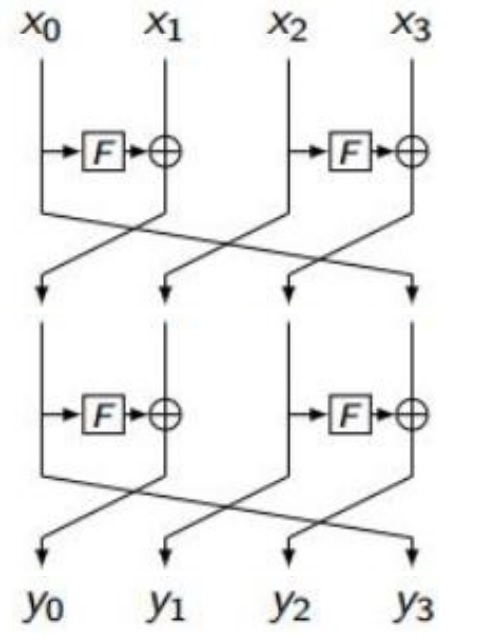
\includegraphics[scale=0.3]{pics/3-2-rounds.jpg}
        \caption{دو دور در \lr{generalized feistel}}
        \label{fig:generalized-feistel:2round}
    \end{figure}
    حال باید بررسی بکنیم که در سه دور چه اتفاقی می‌افتد. در این حالت اگر
    $X_1$
    عوض شود هیچ تغییری در
    $Y_1$
    رخ نمی‌دهد به صورت شکل
    \ref{fig:generalized-feistel:3round}.
    \begin{figure}[H]
        \centering
        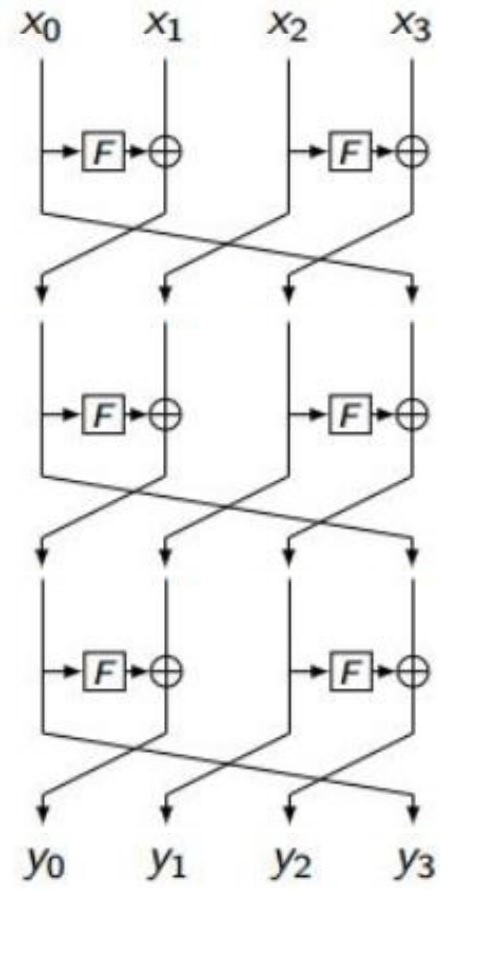
\includegraphics[scale=0.3]{pics/3-3-rounds.jpg}
        \caption{سه دور در \lr{generalized feistel}}
        \label{fig:generalized-feistel:3round}
    \end{figure}
    اما با چهار دور تمامی خورجی‌ها وابسته تمامی ورودی‌ها می‌شوند و دیگر با تغییر حتی یکی
    از ورودی‌ها تمامی خروجی‌ها عوض می‌شود. همچنین من با جست و جو در اینترنت دقیقا یک مقاله پیدا کردم
    که بر روی تعداد جایگشت‌های یک
    \lr{cipher}
    مانند این سوال کار می‌کند که در
    \link{https://d-nb.info/1206696850/34}{اینجا}
    موجود است.
\end{enumerate}
\section{}
در این حالت کافی است که عملا سه بار به توان برسانیم عدد را.
فرض کنید که سه کامپیوتر وجود دارند در شبکه که سه عدد تصادفی و شخصی
$A$ و $B$ و $C$
را برای خودشان می‌سازند. سپس تمامی آن‌ها بر روی اعداد
$q$ و $\alpha$
مانند خود دیفی هلمن دو نفره توافق می‌کنند. سپس هر کدام به ترتیب
$\alpha^A \mod q$ و $\alpha^B \mod q$ و $\alpha^C \mod q$.
سپس هر یک این اعداد را برای کلاینت بعدی خودشان می‌فرستند و آن‌ها نیز عدد دریافتی را برای کلاینت‌های
بعدی خودشان می‌فرستند. پس در حال حاضر اعداد هر کدام از کلاینت‌ها برابر است با:
$\alpha^{CA} \mod q$ و $\alpha^{AB} \mod q$ و $\alpha^{BC} \mod q$.
در نهایت یک بار دیگر نیز هر کدام از این اعداد باید به فرد بعدی فرستاده شود و در نهایت اعداد برابر می‌شوند با:
$\alpha^{ABC} \mod q$ و $\alpha^{BCA} \mod q$ و $\alpha^{CBA} \mod q$.
همان طور که می‌بینید تمامی اعداد یکسان شدند و نتیجه همان کلید ماست.

\noindent
\link{https://en.wikipedia.org/wiki/Diffie\%E2\%80\%93Hellman_key_exchange\#Operation_with_more_than_two_parties}{منبع}
\section{}
\begin{enumerate}
    \item به صورت کلی یک سری کلید در این رمزنگاری وجود دارد که به آن‌ها \lr{weak keys} گفته می‌شود.
    (\link{https://en.wikipedia.org/wiki/Weak_key\#Weak_keys_in_DES}{منبع 1} \link{https://crypto.stackexchange.com/q/12214}{منبع 2})
    از آنجا که
    \lr{DES} از \lr{Feistel Cipher} استفاده می‌کند،
    در صورتی که کلید‌هایی که در
    \lr{key scheduling}
    تولید می‌شود طوری در بیاید که از اول به آخر و آخر به اول یکی باشند عملا الگوریتم
    رمزگذاری و رمزگشایی یکی می‌شود. با توجه به ویکیپدیا این کلید‌ها خاصیت گفته شده را دارند:
    \begin{latin}
    \begin{lstlisting}
0x0101010101010101
0xFEFEFEFEFEFEFEFE
0xE0E0E0E0F1F1F1F1
0x1F1F1F1F0E0E0E0E
0x0000000000000000
0xFFFFFFFFFFFFFFFF
0xE1E1E1E1F0F0F0F0
0x1E1E1E1E0F0F0F0F
\end{lstlisting}
    \end{latin}
    البته دوباره با توجه به ویکیپدیا فقط برخی از پیاده‌سازی‌های خاص باعث می‌شوند که چهار کلید آخر ویژگی گفته شده را داشته باشند.
    \item با توجه به
    \link{https://crypto.stackexchange.com/q/2060}{این}
    دلیل اصلی این انتخاب این بود که اگر مثلا یک
    \lr{CPU}
    خاص دستوری برای انجام دادن
    \lr{3DES}
    داشت بتواند به صورت
    \lr{backward compatible}، \lr{DES}
    را انجام دهد طوری که دو زیر کلید اول را یکی دهد. اما همین الان فهمیدیم که اگر حتی سه بار رمزگذاری نیز
    اتفاق می‌افتاد کافی بود که دو زیر کلید اول یک
    \lr{weak key}
    باشند که رمزگذاری همان رمزگشایی شود. اما مشکل زمانی به وجود می‌آید که سخت افزاری وجود داشته باشد
    که از
    \lr{3DES} دو کلیده
    استفاده می‌کند. این مدل از
    \lr{3DES}
    کاری که می‌کند این است که کلید آخرین رمزنگاری و اولین رمزگاری یکی است و کلید آن رمزگشایی وسط فرق دارد.
    در این حالت در صورتی که هر 3 عملیات ما رمزگذاری بود، در صورتی که می‌خواستیم که
    \lr{DES}
    انجام دهیم مجبور بودیم که یک طوری دو کلید پشت سر هم را
    \lr{weak key}
    انتخاب کنیم که عملا اگر این کار را می‌کردیم، بایستی تمامی کلید‌هایمان را
    \lr{weak}
    انتخاب می‌کردیم. اما از اول رمزگذاری کنیم بعد رمزگشایی و بعد رمزنگاری در صورتی که تمامی
    زیر کلید‌ها را یکی بدهیم عملا فقط یک مرحله رمزگذاری انجام می‌شود
    (رمزنگاری اول با رمزگشایی دوم خنثی می‌شود)
    و در نتیجه می‌توان
    \lr{DES}
    را پیاده سازی کرد.

    همچنین یک مورد دیگر که به آن می‌توان اضافه کرد این است که ممکن است که اگر سه تا رمزنگاری پشت سر هم داشتیم
    به صورت اشتباهی دو
    \lr{weak key}
    را پشت سر هم قرار دهیم و عملا
    \lr{3DES} تبدیل به \lr{DES}
    شود.
\end{enumerate}
\section{}
\begin{enumerate}
    \item خیر این کار امنیتی برای ما تامین نمی‌کند.
    فرض کنید که سه پیام
    $M_1, M_2, M_3$ که هر کدام به طول $n$ بلوک هستند داریم.
    همچنین ما
    \lr{CBC-MAC}
    پیام‌های
    $M_1, M_2$ و $M_1 || n || M_3$ را در اختیار داریم که آن‌ها را به ترتیب
    $C_1, C_2, C_3$ می‌نامیم.
    (در اینجا $||$ نشان دهنده‌ی \lr{concat} شدن پیام‌ها به هم است.)
    دقت کنید که عملا زمانی که در حال حساب کردن
    $\operatorname{MAC}(M_1 || n || M_3)$
    هستیم زمانی که تا
    $M_1 || n$
    حساب کرده‌ایم جوابمان عملا همان
    $C_1$
    است. حال کاری که لازم است بکنیم این است که بلوک بعدی در حال حساب کردن مک را بدین صورت قرار دهیم:
    $C_1 \oplus C_2 \oplus M_3[0]$ که $M_3[0]$
    می‌شود اولین بلوک
    $M_3$.
    کاری که در اینجا کردیم این است که جواب نهایی که
    \lr{MAC}
    بدست می‌آورد عملا برای
    $\operatorname{MAC}(M_2 || n || M_3)$
    است.

    \link{https://crypto.stackexchange.com/a/11152}{منبع 1} \link{https://crypto.stackexchange.com/a/31859}{منبع 2}
    \item یک نکته‌ی بدی که در این حالت وجود دارد این است که آخرین بلوک خروجی
    \lr{ciphertext}
    که عملا دست مهاجم هم قرار دارد همان نتیجه‌ی
    \lr{CBC-MAC}
    است قبل از اینکه با
    $k_2$
    رمز شود. پس اگر بخواد که مهاجم مک را عوض کند یا اینکه باید کاری بکند که آخرین خانه‌ی
    \lr{CBC Cipher}
    ثابت بماند یا اینکه کلا رمزنگاری با
    $k_2$
    را معکوس کند که امکان پذیر نیست. پس به نظر من این مدل مشکلی ندارد.
    % https://en.wikipedia.org/wiki/CBC-MAC#Encrypt-last-block this uses two keys!
\end{enumerate}
\section{}
\begin{enumerate}
    \item به صورت خلاصه دلیل آن این است که تنها علی می‌تواند
    $r$
    را امضا کند و
    $r$
    را نیز فاطمه ساخته است. پس قطعا علی تمامی پیام‌ها را دارد می‌فرستد.
    \item مهاجم می‌تواند که
    $S(r)$
    را با حساب کردن
    $s \oplus h(m \oplus r)$
    بدست بیاورد. حال برای عوض کردن پیام کافی است که
    به جای
    $s$
    قرار دهد
    $s \oplus h(m \oplus r) \oplus h(m' \oplus r)$
    و آن را به عنوان امضا ارسال کند.
    \item به نظر من یک کار خوبی که می‌توان کرد این است که امضایی که فرستاده می‌شود را برابر عبارت
    $S(h(m) \oplus h(r))$
    قرار دهیم. در این حال در صورتی که یک مهاجم بخواد امضا را جعل کند باید کاری کند که
    $h(m) = h(m')$
    بشود که
    $h(m) \oplus h(r) = h(m') \oplus h(r)$ و در نهایت $S(h(m) \oplus h(r)) = S(h(m') \oplus h(r))$
    را نتیجه بدهد. و از آن‌جا که یکی از ویژگی‌های تابع هش باید این باشد که دقیقا پیدا کردن دو
    $m$ و $m'$
    سخت باشد به صورتی که
    $h(m) = h(m')$
    باشد پس مهاجم کاری نمی‌تواند بکند.
\end{enumerate}
\section{}
\begin{enumerate}
    \item کد مورد نظر در فایل ژوپیتر پیوست شده موجود است.
    \item برای RSA از کلید‌‌های ۲۰۴۸ بیتی استفاده کردم و برای AES از ۲۵۶ بیتی.
    دلیل استفاده از این طول کلید برای RSA را از
    \link{https://www.jscape.com/blog/should-i-start-using-4096-bit-rsa-keys}{اینجا}
    برداشتم و برای
    AES
    نیز این بیشترین طول کلید بود که وجود داشت.
    \item با توجه به داکیونت و بولت‌هایی که وجود دارد می‌توان الگوریتم‌های زیر را از آن در آورد:
    \begin{itemize}
        \item \textbf{\lr{XEdDSA}:} با توجه به چیزی که من خواندم الگورتم \lr{key agreement}ای
        وجود دارد به اسم
        \link{https://cryptography.io/en/latest/hazmat/primitives/asymmetric/x25519/}{X25519}
        که تا حدودی شبیه دیفی هلمن عمل می‌کند. کاری که این الگوریتم
        \lr{XEdDSA}
        انجام می‌دهد این است که می‌تواند به کمک کلید‌هایی که
        \lr{X25519}
        می‌سازد
        \lr{digital signature}هایی
        انجام دهد که شبیه الگوریتم
        \link{https://en.wikipedia.org/wiki/EdDSA}{EdDSA}
        است. در کل برای امضای دیجیتال این الگوریتم استفاده می‌شود.
        \item \textbf{\lr{X3DH}:} یک الگوریتم \lr{key agreement}
        است که دو نفر مقابل می‌توانند به کمک کلید‌های عمومی و خصوصی خود از صحت و دستکاری نشدن کلید به اشتراک گذاشته شده
        مطمئن شوند. این الگوریتم
        \lr{forward secrecy}
        نیز دارد پس اگر یکی از کلید‌ها لو برود، کلید‌های دیگر لو نمی‌رود.
        یک نکته‌ای که وجود دارد این است که این الگوریتم
        \lr{asynchronous}
        است. یعنی اینکه لازم نیست طرف مقابل آنلاین باشد که اول تبادل کلید انجام شود و سپس پیام‌ها بتوانند ارسال شوند.
        \item \textbf{\lr{PQXDH}:} این دقیقا مثل \lr{X3DH} است ولی برای زمانی که کامپیوتر‌های کوانتمی به جای کامپیوتر‌های عادی آمده‌اند.
        \item \textbf{\lr{Double Ratchet}:} طبق چیزی که من از \link{https://en.wikipedia.org/wiki/Double_Ratchet_Algorithm}{ویکیپدیا}
        خواندم این الگوریتم کاری که می‌کند این است که از یک کلید شروع می‌کند و یک دنباله از کلید‌ها می‌سازد. نکته‌آی که درباره‌ی این کلید‌ها
        وجود دارد این است که از یک کلید می‌توان به کلید‌های بعدی‌اش رسید ولی به کلید‌‌های قبلی نمی‌توان رسید.
        یعنی اگر آخرین کلید سشن ما لو رفت کافی است که کلید را عوض کنیم کلا و اصلا نیازی نیست که نگران کلید‌‌های قبلی باشیم.
        \item \textbf{\lr{Sesame}:} این الگوریتم برای مدیریت کردن \lr{double ratchet} که در قسمت قبل بود و کلید‌های نشستی که
        \lr{X3DH}
        درست کرده است استفاده می‌شود.
        \item \textbf{\lr{AES} و \lr{HMAC}:} سیگنال پیشنهاد می‌کند که پیام‌ها با الگوریتم
        \lr{AES} با مود \lr{CBC}
        رمز بشوند. همچنین از
        \lr{HMAC-SHA256} یا \lr{HMAC-SHA512}
        استفاده می‌شود برای چک کردن دست نخوردن پیام.
        \link{https://signal.org/docs/specifications/doubleratchet/\#recommended-cryptographic-algorithms}{منبع}
    \end{itemize}
    \item زمانی که توافق کلید انجام می‌شود اتفاقی که می‌افتد این است که هر شخص در حال تماس
    \lr{SHA256} عدد $g^a$ (از الگوریتم دیفی هلمن)
    را حساب می‌کنند و جواب آن به ۴ قسمت ۶۴ بیتی تقسیم می‌شود. تلگرام ۳۳۳ تا اموجی برای این موضوع تایین کرده است که با 
    یک باقی مانده گیری ساده از هر کدام از قسمت‌ها می‌توان به اموجی مورد نظر رسید و آن را برای کاربر نمایش داد.
    مشکلی که اینجا پیش می‌آید این است که به احتمال ۱۰۰ درصدی جلوی حملات مرد میانی را نمی‌گیریم چرا که ممکن است باقی مانده‌های ما یکی
    شود در حالی که کلید یکی نشد. اما تلگرام ادعا می‌کند که احتمال این اتفاق
    \lr{0.9999999999}
    است.

    یک نکته‌ای که در اینجا وجود دارد این است که تلگرام از الگورتمی شبیه الگوریتم دیفی هملن (و بر پایه آن)
    و نه خود دیفی هلمن استفاده می‌کند. مثل خود دیفی هلمن در ابتدا هر دو شخص باید بر روی اعداد
    $g$ و $n$
    توافق می‌کنند. همچنین
    $a$ و $b$
    سیکرت هستند.
    مراحل این رمزنگاری بدین صورت هستند:
    \begin{enumerate}
        \item شخص A به B 
        در ابتدا
        $\operatorname{SHA256}(g^a \mod n)$
        را حساب کرده و می‌فرستند.
        \item شخص B به A
        $g^b \mod n$
        را حساب کرده و می‌فرستند.
        \item در اینجا تازه A به B
        $g^a \mod n$
        را حساب کرده و می‌فرستند.
        همچنین
        $(g^b)^a \mod n$
        را نیز حساب می‌کند و به عنوان کلید استفاده می‌کند.
        \item B
        چک می‌کند که آیا هشی که در ابتدا
        A به B
        فرستاده بود همان برابر هش عددی است که در حال حاضر دریافت می‌کند یا خیر. در صورتی که برابر نبود تماس را متوقف می‌کنیم.
        در غیر این صورت این شخص نیز
        $(g^a)^b \mod n$
        را حساب می‌کند و به عنوان کلید رمزنگاری استفاده می‌کند.
    \end{enumerate}
    در کل دلیل استفاده از اموجی و موارد مشابه برای راستی آزمایی کلید برای این موضوع است که یک حمله‌ی مرد میانی می‌تواند انجام بگیرد.
    در صورتی که حمله مرد میانی انجام بگیرید کلیدی که بین دو طرف قرار دارد متفاوت می‌شود و در نتیجه اموجی‌ها نیز متفاوت می‌شود.
    طبق چیزی که داک تلگرام نوشته است دلیل استفاده از تابع
    \lr{SHA256}
    برای این است که حمله کننده فقط یک شانس برای جعل کرد رمزی دارد که اموجی‌های یکسانی درست کند.
\end{enumerate}
\end{document}
